\chapter{Analisi Ammortizzata}
Nell'analisi ammortizzata il tempo richiesto per eseguire una serie di operazioni \textit{n} su una struttura dati viene calcolato come media dei tempi di tutte le operazioni eseguite. Questo tipo di analisi si può utilizzare per dimostrare che il costo medio di un'operazione è piccolo se si considera la media di una sequenza di operazioni anche se magari un'operazione all'interno della sequenza è particolarmente costosa. In caso di analisi ammortizzata non utilizziamo teoria delle probabilità, bensì valutiamo le prestazioni media di ciascuna operazione nel caso peggiore.\\
Per effettuare queste analisi saranno considerati due esempi in particolare:
\begin{enumerate}
    \item \textbf{Stack Multipop}: uno stack in cui, oltre che le operazioni classiche di pop e push con costo O(1), troviamo un'operazione chiamata \textbf{Multipop(S, k} che effettua, sullo stack S, k pop. Questa operazione avrà come costo $O(min(|S|,k))$ poiché, se lo stack è vuoto, l'operazione terminerà prima e si fermerà al numero di elementi presenti nello stack.
    \begin{algorithmic}[1]
        \Statex \textbf{Multipop($S, k$)}
        \While{$\neg \text{StackEmpty}(S) \ \textbf{and} \ k > 0$}
            \State $Pop(S)$
            \State $k \gets k - 1$
        \EndWhile
    \end{algorithmic}
    \item \textbf{Contatore binario con incremento}: questo sarà un array di k elementi che rappresenteranno, dalla cifra più significativa alla cifra meno significativa, un numero che potrà essere al più $2^k-1$. Questo contatore avrà una sola operazione che è \textbf{increment} che non fa altro che aumentare il contatore binario di uno. Nel caso in cui tutti gli elementi dell'array siano 1, cioè abbiamo raggiunto il numero massimo disponibile, effettuando increment il contatore si resetterà con tutti i bit a 0. Questo caso è lo scenario più costoso e la sua complessità è in O(k).
    \begin{samepage}
    \begin{algorithmic}[1]
        \Statex \textbf{Increment($A$)}
        \State $i \gets 0$
        \While{$i < A.\text{length} \ \textbf{and} \ A[i] = 1$}
            \State $A[i] \gets 0$
            \State $i \gets i + 1$
        \EndWhile
        \If{$i < A.\text{length}$}
            \State $A[i] \gets 1$
        \EndIf
    \end{algorithmic}
    \end{samepage}
\end{enumerate}
Un modo naturale di calcolare la complessità di una sequenza di operazioni $n$ è quello di:
\begin{enumerate}
    \item Calcolare il caso pessimo di una singola operazione;
    \item Moltiplicare il costo per $n$.
\end{enumerate}
Per quanto questo approccio dia sicuramente una stima corretta, questa è fin troppo pessimistica. Se guardiamo, infatti, una sequenza di operazioni su di uno stack multipop, noteremo che la singola operazione ha complessità $O(n)$ dato che non posso fare più pop di quanti push ho effettuato e, quindi, il costo di $n$ operazioni sarà di $O(n^2)$. Allo stesso modo, avremo che per l'incremento del contatore binario, la complessità della singola operazione è $O(k)$ e, dunque, la complessità di $n$ operazioni sarebbe $O(nk)$. Vedremo adesso come questa stima sia sovrabbondante e possiamo renderla più precisa tramite un'ulteriore analisi.

\section{Metodo dell'aggregazione}
L'analisi basata sul metodo dell'aggregazione dimostra che, per ogni $n$, una sequenza di operazioni $n$ impiega, nel caso peggiore, un tempo totale $T(n)$ e, quindi, il \textbf{costo ammortizzato} per operazione è $T(n)/n$. Avremo dunque la necessità di calcolare $T(n)$ in maniera diretta analizzando le operazioni passo dopo passo.
\vspace{0.5em}
\subsection{Stack MultiPop}
Consideriamo ora il caso dello \textit{stack multipop}.  
Supponiamo di avere una sequenza di $n$ operazioni del tipo:
\[\langle op_1, \dots, op_n \rangle \xleftarrow{} \{\text{pop}, \text{push}, \text{multipop}\}.\]
Possiamo espandere ogni operazione \texttt{multipop} sostituendola con una serie di \texttt{pop}, ottenendo così una nuova sequenza:
\[\langle op'_1, \dots, op'_m \rangle \xleftarrow{} \{\text{pop}, \text{push}\}.\]
Naturalmente, queste due sequenze avranno la stessa complessità totale.  
Osserviamo che, in ogni prefisso della sequenza,
\[\#\text{Pop}(\langle op'_1, \dots, op'_m \rangle) \leq \#\text{Push}(\langle op'_1, \dots, op'_m \rangle)=\#\text{Push}(\langle op_1, \dots, op_n \rangle)\leq n.\]

Pertanto:
\[\#\text{Pop}(\langle op'_1, \dots, op'_m \rangle) \leq n.\]
Sia dunque $\langle op_1, \dots, op_n \rangle$ la sequenza \textbf{più costosa}.
Allora:
\begin{align*}
T(n) &= \text{costo}(\langle op_1, \dots, op_n \rangle) \\
     &= \text{costo}(\langle op'_1, \dots, op'_m \rangle) \\
     &= \#\text{Pop}(\langle op'_1, \dots, op'_m \rangle)
      + \#\text{Push}(\langle op'_1, \dots, op'_m \rangle) \\
     &\leq n + n = 2n.
\end{align*}
Di conseguenza, il costo ammortizzato per operazione è:
\[\frac{T(n)}{n} \leq \frac{2n}{n} = 2.\]
\subsection{Contatore binario}
Considerando invece il caso del \textbf{contatore binario}, notiamo quanto segue in figura: 
\begin{figure}[H]
    \centering
    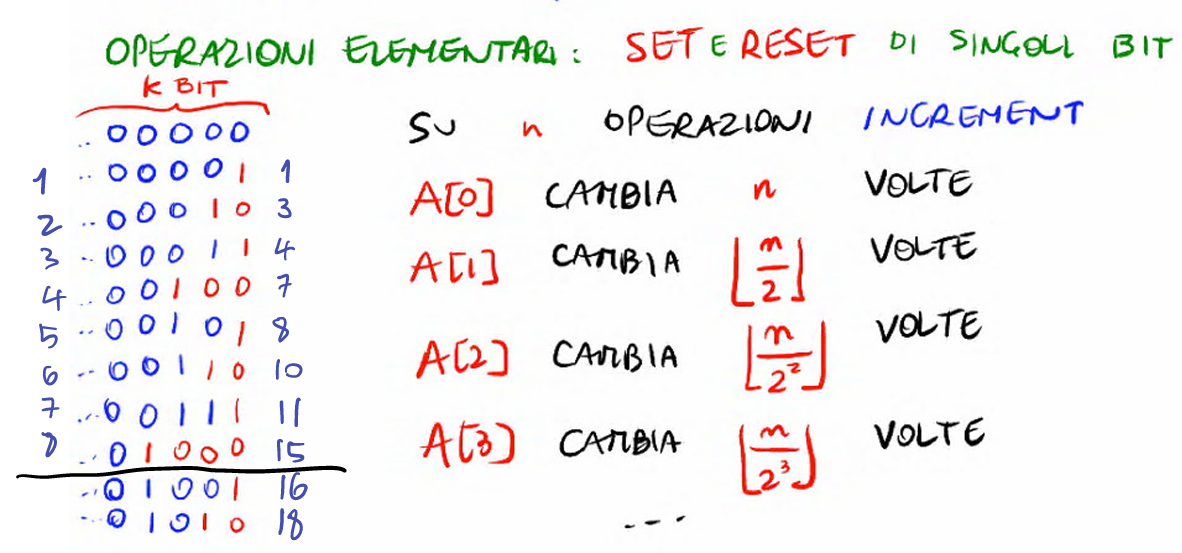
\includegraphics[width=0.8\linewidth]{Images/capitolo_1_2/contatore_binario_cambi.png}
    \caption{Cambi dei bit a ogni incremento}
    \label{fig:cambi_bit_incremento}
\end{figure}

Notiamo quindi come possiamo calcolare:
\begin{align*}
T(n) 
  &= n + \left\lfloor \frac{n}{2} \right\rfloor 
     + \dots 
     + \left\lfloor \frac{n}{2^{k-1}} \right\rfloor \\
  &= \sum_{i=0}^{k-1} \left\lfloor \frac{n}{2^i} \right\rfloor 
   \leq \sum_{i=0}^{k-1} \frac{n}{2^i} 
   < \sum_{i=0}^{\infty} \frac{n}{2^i} \\
  &= n \sum_{i=0}^{\infty} \frac{1}{2^i} 
   = n \cdot 2 = 2n.
\end{align*}\footnote{Il risultato è ottenuto dal fatto che è una serie geometrica.}

Per cui il costo ammortizzato per operazione è: $\frac{T(n)}{n} < \frac{2n}{n} = 2$.

\section{Metodo dell'accantonamento}
Il metodo degli accantonamenti comincia adesso ad utilizzare l'idea di \textbf{ammortizzare} i costi su più operazioni e ciò viene fatto in maniera tale che valga:
\[T(n) = \sum_i^nc_i \leq \sum_i^nc'_i\]

Dove $c'_i$ rappresenta il costo ammortizzato che stiamo definendo e $c_i$ rappresenta il costo reale. Se vale $c'_i>c_i$ allora quello che faremo sarà consumare $c_i$ per il reale costo dell'operazione e il restante "credito", lo terremo da parte per ammortizzare i costi di altre operazioni. Nel caso contrario in cui $c_i > c'_i$, la differenza di crediti per eseguire quella specifica operazione sarà recuperata dai crediti conservati. 

Sia $D_0$ la configurazione iniziale di una struttura dati, siano $op_1, ..., op_n$ una sequenza di operazioni, e sia $D_i \xrightarrow{op_i}D_{i+1}$ la configurazione della struttura dati dopo l'operazione $i$-esima. Supponiamo che $\forall j = 0,...,n-1$ su $D_j$ sia sempre immagazzinata una quantità di costi pari almeno a $c_{j+1}-c_{j+1}$, la quantità di costi immagazzinata in $D_j$ è uguale a: 
\begin{align*}
D_j
    &=\sum_{i=1}^j (c'_i-c_i) = \sum_i^jc'_i-\sum_i^jc_i \\
    \text{E quindi da}\\
    &c_{j+1}-c'_{j+1} \leq \sum_i^jc'_i-\sum_i^jc_i\\
    \text{Otteniamo}\\
    &0 \leq \sum_i^jc'_i-\sum_i^jc_i \\
    \text{Per cui avremo che}\\
    &\sum_i^{j+1}c_i\leq \sum_i^{j+1}c_i' \xrightarrow{} \sum_i^{n}c_i\leq \sum_i^{n}c_i' 
\end{align*}

\subsection{Stack MultiPop}
Per utilizzare il metodo dell'accantonamento nel caso di uno stack con multipop, l'idea è quella di fornire un credito ammortizzato di 2 all'operazione di push. Per cui, un credito lo utilizziamo per il costo reale dell'operazione di push, il restante credito lo utilizzeremo per effettuare l'operazione di pop che, di conseguenza, avrà un costo ammortizzato di 0. Da qui segue:
\begin{align*}
    &c'_{push} = 2 \quad c'_{pop}= 0 \\
    &\sum_i^jc_i'-\sum_i^jc_i = |S_j| \geq 0 \\
    &\sum_i^jc_i\leq\sum_i^jc_i' \xrightarrow{} \sum_i^nc_i\leq\sum_i^nc_i' = 2*num_{push}\leq 2
\end{align*}
\subsection{Contatore binario}
Come già fatto prima, anche in questo caso possiamo assegnare ad ogni operazione di set un costo ammortizzato di 2 di cui uno verrà utilizzato per effettuare l'operazione di set e l'altro per l'operazione di reset. In base a ciò, sappiamo che il costo ammortizzato di un operazione di increment sarà $\leq$ di 2 poiché al massimo può esserci una sola operazione di set. \footnote{Il minore c'è perché quando il contatore raggiunge il suo valore massimo e vengono fatte solo operazioni di reset si utilizza solo il credito accumulato.} 
Effettuando l'analisi:
\begin{align*}
    &c'_{set} = 2 \quad c'_{reset} = 0 \\
    &\sum_i^jc'_i - \sum_i^jc_i = \text{\# bit uguali ad 1}\\
    &\sum_i^nc'_i \geq \sum_i^nc_i \xrightarrow{} \sum_i^nc_i \leq \sum_i^nc_i'\leq 2n
\end{align*}

\section{Metodo del potenziale}
Il metodo del potenziale risulta essere un caso generico del metodo dell'accantonamento. Questa volta, anziché assegnare un costo ammortizzato alle singole operazioni, andremo a generare una \textbf{funzione potenziale $\phi$} che conserva i crediti dell'intera struttura dati assegnando ad ogni configurazione $D_i$ un numero reale. Definiamo: 
\begin{align*}
    &D \xrightarrow{\phi}\phi(D)\in R\\
    &c'_i = c_i+\phi(D_i)-\phi(D_{i-1})\\
    &\Delta\phi_i = \phi(D_i)-\phi(D_{i-1}) \quad \text{ Variazione di potenziale}
\end{align*}

Possiamo continuare:
\begin{align*}
    &\sum_i^n c'_i = \sum c_i+\phi(D_i)-\phi(D_{i-1})\\
    &=c_1+(\phi(D_1)-\phi(D_0)) + c_2+ (\phi(D_2)-\phi(D_1))+...+\\&...+c_{n-1}+\phi(D_{n-1})-\phi(D_{n-2})+c_n + (\phi(D_{n})-\phi(D_{n-1})\\
    &=\sum_i^n c_i+ (\phi(D_n)-\phi(D_0))\\
    &\text{Segue:}\\
    &\sum_i^n c'_i = \sum_i^n c_i + \phi(D_{n})-\phi(D_{0})\\
    &\text{Per cui avremo che:}\\
    &\sum_i^n c'_i \geq \sum_i^n c_i \xrightarrow{} \sum_i^n c_i + \phi(D_{n})-\phi(D_{0}) \geq \sum_i^n c_i\\
    &\phi(D_n) \geq \phi(D_0)  \xrightarrow{implica} \sum_i^n c_i' \geq \sum_i^n c_i  \\
    &\text{Che sono in genere le funzioni potenziali che riteniamo più utili.}
\end{align*}

\subsection{Stack Multipop inizialmente vuoto}
La funzione potenziale $\phi$ che utilizzeremo sarà $\phi(S) = |S|$ se $S_0$ è lo stack vuoto, avremo che $\phi(S_0) = 0$, quindi avremo che $\phi(S) \geq \phi(S_0)$. \footnote{Nel caso in cui questa condizione non valga, avremo che il risultato della nostra analisi avrà, oltre che n, una costante.} Analizziamo adesso i costi uno ad uno:
\begin{align*}
    &c'_{pop}= c_{pop} + \phi(S_i) - \phi(S_{i-1}) = 1+|S_i| - |S_{i-1}| = 0 \text{ in quanto } |S_i| = |S_{i-1}|+1\\
    &c'_{multipop} = c_{multipop} + \phi(S_i) - \phi(S_{i-1}) = 0 \text{ per lo stesso motivo di prima}\\
    &c'_{push} = c_{push} + \phi(S_i) - \phi(S_{i-1}) = 1+1=2\\
    &\text{Per tanto: } \sum_i^nc_i\leq \sum_i^nc'_i=2*num_{push}\leq 2n
\end{align*}

\subsection{Stack Multipop non vuoto}
Cerchiamo adesso di fare i calcoli con uno stack multipop per cui però $\phi(D_0)!=0$.
\begin{align*}
    &\sum_i^nc'_i = \sum_i^nc_i+\phi(Dn)-\phi(D_0)\\
    &\sum_i^nc_i = \sum_i^nc_i' - \phi(Dn)+\phi(D_0)\\
    &= \sum_i^nc_i' - |S_n| + |S_0| \\
    &\leq \sum_i^nc_i'+|S_0| \leq 2n+ |S_0|\\
    &\text{Da cui avremo una complessità di $O(n+|S_0|)$}
\end{align*}

\subsection{Contatore binario inizialmente nullo}
Scegliamo in questo caso la funzione potenziale come $\phi(D_i) = \text{\# bit uguali ad 1}$. Visto che il contatore è inizialmente nullo avremo che $\phi(D_0) = 0$ per cui $\phi(D_i) \geq \phi(D_0)$.

\begin{align*}
    &c'_i = c_i + \phi(D_i) - \phi(D_{i-1})\\
    &c_i = num_{set_i} + num_{reset_i} \\
    &\Delta\phi_i = num_{set_i} - num_{reset_i}\\
    &\text{Pertanto avremo che:}\\
    &c_i' = c_i + \Delta\phi_i = (num_{set_i} + num_{reset_i}) + (num_{set_i} - num_{reset_i}) = 2*num_{set_i} \leq 2\\
    &\text{Da cui:}\\
    &\sum_i^nc_i \leq \sum_i^n c_i' = 2* \sum_i^n num_{set_i} \leq 2n
\end{align*}

\subsection{Contatore binario inizialmente non nullo}
Come per lo stack multipop, proviamo a fare i conti per un contatore inizialmente non nullo. 
\begin{align*}
    &\sum_i^nc_i = \sum_i^nc'_i - \phi(D_n)+\phi(D_0) \leq 2n+\phi(D_0) \leq 2n+k \\
\end{align*}
Se $k=O(n)$ allora avremo che $2n+k=O(n) \xrightarrow{}\sum_i^n c_i = O(n+k)$

\section{Tabelle dinamiche}
Le tabelle dinamiche sono delle tabelle che aumentano e diminuiscono la loro dimensione per risolvere problemi overflow e di underflow. Sia $T$ una tabella diremo che:
\begin{itemize}
    \item \textbf{size[T]:} dimensione della tabella;
    \item \textbf{num[T]:} numero di elementi in T;
    \item \textbf{$\alpha(T)$:} una funzione che restituisce $\frac{num[T]}{size[T]}$ se size[T]$>$0, 1 altrimenti. Questo valore sarà il \textbf{fattore di carico}.
\end{itemize} 

L'inserimento nel caso in cui il fattore di carico sia 1, cioè la tabella è piena, farà sì che la tabella aumenterà le sue dimensioni del doppio. In termini di implementazione, verrà creata una nuova tabella con dimensioni doppie rispetto alla prima e gli elementi verranno ricopiati al suo interno aggiungendo anche l'ultimo da inserire. Partendo convenzionalmente con una tabella di dimensione 0, vediamo che gli inserimenti $2^i+1$ sono i più costosi poiché sono quelli in cui la tabella è piene e si necessita una espansione. 
Analizziamo la complessità in termini di inserimenti elementari. Sia $n=2^k$ il numero di inserimenti, sappiamo che l'inserimento più costoso è il $2^{k-1}+1\text{-Esimo}$ con costo $2^{k-1}+1 = n/2+1$\footnote{Il costo $2^{k-1}$ è quello derivante dalla copia dell'array.}
\subsection{Analisi mediante metodo dell'aggregazione}
Andando ad analizzare il costo delle operazioni mediante il metodo dell'aggregazione, partiamo tenendo conto di come ogni operazione di inserimento abbia costo 1 nel caso in cui questo la tabella abbia posizioni disponibili mentre il costo è $i$ se $i-1$ è una potenza di 2. Per cui, eseguendo i calcoli avremo:
\begin{align*}
    T(n) = \\
    &\sum_i^nc_i = (2^0+2^1+...+2^{\lfloor lg(n-1) \rfloor }+n=\\
    &= (2^{\lfloor lg(n-1) \rfloor+1}-1+n \leq 2^{lg(n-1)+1}-1+n\\
    &= 2(n-1)-1+n = 3n-3 = O(n)\\
    \\
    &\text{per cui, il costo ammortizzato sarà:}\\
    &c'_i = \frac{3n-3}{n} = O(1)
\end{align*}

\subsection{Analisi mediante metodo degli accantonamenti}
Come ipotesi di costo ammortizzato possiamo utilizzare 3 per cui:
\begin{itemize}
    \item 1 unità servirà per il costo reale dell'inserimento;
    \item 1 unità per pagare il costo della propria copia;
    \item 1 unità per pagare il costo di copia di un elemento che è già stato ricopiato. 
\end{itemize}
L'idea è che ad ogni espansione, avremo nessun elemento precedentemente inserito avrà credito per la successiva copia. Il numero di elementi che necessita di crediti per la successiva copia all'i-esimo inserimento inserimento sono $2^{i-1}$ per cui dividiamo questo credito nei successivi inserimenti che sono $2^{i+1}-2^i=2^i$. Per cui ci basterà dividere $2^i/2^{i-1}$ e avremo che ad ogni inserimento dovremo accumulare 2 crediti, uno per la copia dell'elemento appena inserito e 1 per gli elementi precedenti.
Per fissare meglio il concetto di quello che succede, possiamo vedere il seguente schema.
\begin{figure}
    \centering
    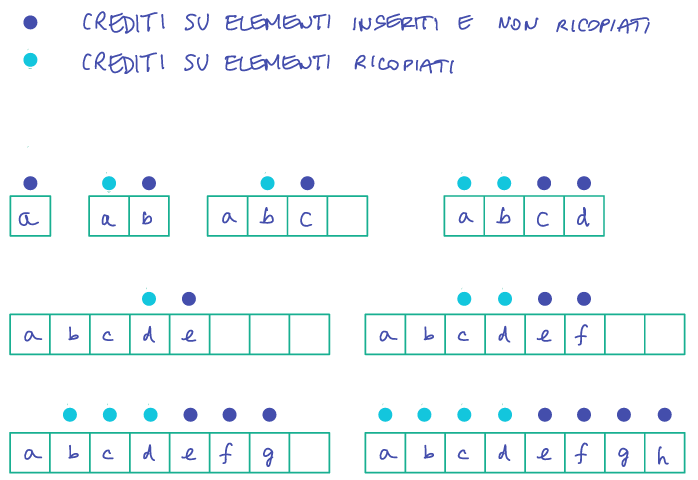
\includegraphics[width=0.5\linewidth]{Images/capitolo_1_2/schema_inserimenti_tabella.png}
    \caption{Utilizzo dei gettoni per copia}
    \label{fig:inserimenti_su_tabella}
\end{figure}
Osserviamo che $\sum_i^n c'_i \geq \sum_i^n c_i$ per cui $T(n)\leq 3n$.
Analizzando il numero di crediti che abbiamo vedremo:
\begin{align*}
    &\# crediti = \#copia\_precedente+\#copia\_inserito\\
    &= 2*\#copia\_inserito = 2*(num[T]-1/2size[T])=2num[T] -size[T]
\end{align*}

\subsection{Analisi con il metodo del potenziale}
Definiamo adesso la funzione potenziale sfruttando quanto fatto prima. Sappiamo che sono necessari $2num[T] - size[T]$ crediti. Per cui la nostra funzione potenza sarà:
\[\phi(T) = 2num[T] - size[T]\]
Possiamo notare anche qui come $\phi(T_0) = 0$ nel caso in cui la tabella sia ancora vuota e, poiché $1/2 size[T] \leq num[T]$, avremo che $\phi(T)\geq0 = \phi(T_0)$. Sulla base di questo possiamo analizzare i costi reali degli inserimenti:
\begin{align*}
    &\text{Caso senza espansione}\\
    \\
    &c'_{ins} = c_{ins}+\phi(T_i)-\phi(T_{i-1})\\
    &=1+(2*n_i-s_i)-(2n_{i-1}-s_{i-1}) = 1+2 = 3.
    \\
    &\text{Caso con espansione}\\\\
    &c'_{ins} = c_{ins}+\phi(T_i)-\phi(T_{i-1})\\
    &=n_i+(2n_i-s_i)-(2n_{i-1}-s_{i-1}) \quad \text{Ricordando che $S_{i-1}=n_i-1$}\\ 
    &=3\\\\
\end{align*}

\subsection{Tabelle dinamiche con cancellazione}

Consideriamo adesso le tabelle dinamiche che possono effettuare anche operazioni di cancellazione di elementi. Immaginando di non voler mai far scendere il fattore di carico sotto di $1/2$, accettando quindi di avere al massimo metà spazio inutilizzato, ad ogni cancellazione che farebbe scendere il fattore di carico sotto 1/2 avverrebbe un'operazione di contrazione. Immaginiamo lo scenario in cui, dopo aver riempito la tabella, inseriamo un altro elemento per aumentare la dimensione della tabella. Dopodiché cancelliamo due elementi causando una contrazione e poi così in loop. Questo sarebbe naturalmente lo scenario peggiore che causerebbe un grosso problema in termini di complessità.
\begin{figure}[H]
    \centering
    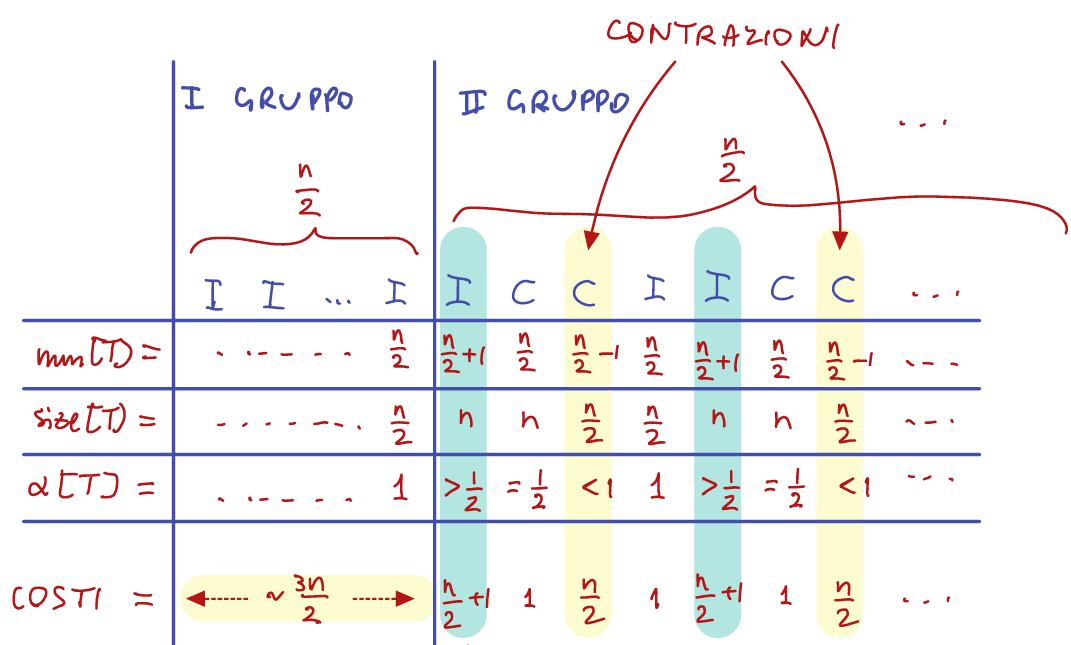
\includegraphics[width=0.8\linewidth]{Images/capitolo_1_2/schema_tabella_dinamica.png}
\end{figure}

Analizziamo la complessità di questo processo:
\begin{align*}
    &3*n/2 \quad \text{Costo dei primi n/2 operazioni}\\
    &+1/4*n/2*(n/2+1) \quad \text{Inserimenti con espansione II gruppo}\\
    &+1/4*n/2*(n/2) \quad \text{Cancellazione con contrazione II gruppo}\\
    &+ 2/4 *n/2 \quad \text{Inserimenti e cancellazioni semplici II gruppo}
\end{align*}

Sommando tutto abbiamo una complessità di circa $n^2$. Il problema di questo processo è il fatto che, quando avviene una contrazione subito dopo un'espansione, non abbiamo il tempo per accumulare crediti. Per cui, ci accontenteremo di avere $\alpha(T) \ge 1/4$. Utilizziamo il metodo del potenziale per fare un analisi di questi casi. Poniamo:

\begin{equation*}
\phi(T)=
    \begin{cases}
        2num[T]-size[T] \text{ se $\alpha[T]>1/2$}\\
        1/2size[T]-num[T] \text{ se $\alpha[T]\le1/2$} \\
    \end{cases}
\end{equation*}

È importante notare che se $\alpha(T) = 1/2$ entrambe valgono zero, rendendo la funzione potenziale continua. Inoltre vale sempre $\phi(T)\ge\phi(T_0)=0$. 
Analizziamo i vari casi di inserimento e cancellazione sulla base di questo schema:
\begin{figure}[H]
    \centering
    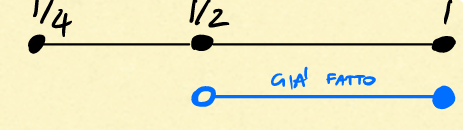
\includegraphics[width=0.5\linewidth]{Images/capitolo_1_2/schema_casi_inserimento.png}
\end{figure}
\textbf{Caso $1/4 \le \alpha(T)<1/2$}
\begin{align*}
    &c_i'=c_i+\phi(T_i)-\phi(T_{i-1})\\
    &=1+(1/2s_i-n_i)-(1/2s_{i-1}-n_{i-1})\\
    &=1+1/2s_{i-1}-n_{i-1}-1-1/2s_{i-1}+n_{i-1}=0
\end{align*}
\textbf{Caso $\alpha(T)=1/2$}
\begin{align*}
    &c_i'=c_i+\phi(T_i)-\phi(T_{i-1})\\
    &=1+(2n_i-s_i)-(2n_{i-1}-s_{i-1})\\
    &= 1+2(n_{i-1}+1-s_{i-1}-2n_{i-1}+s_{i-1})= 3
\end{align*}

Gli stessi casi sono da considerarsi per le cancellazioni.
\textbf{Caso $1/2 < \alpha(T)\le1$}
\begin{align*}
    &c'_c= c_c+\phi(T_i)-\phi(T_{i-1})\\
    &=1+(2n_i-s_i)-(2n_{i-1}-s_{i-1})\\
    &=1+2n_{i-1}-2-s_{i-1}-2n_{i-1}+s_{i-1}=-1
\end{align*}
\textbf{Caso $1/4 \le \alpha(T)<1/2$}
\begin{align*}
    &c'_c= c_c+\phi(T_i)-\phi(T_{i-1})\\
    &=1+(1/2s_i-n_i)-(1/2s_{i-1}-n_{i-1})\\
    &=1+1/2s_{i-1}-n_{i-1}+1-1/2s_{i-1}+n_{i-1} = 2
\end{align*}
\textbf{Caso $\alpha(T)=1/4$}
\begin{align*}
    &c'_c= c_c+\phi(T_i)-\phi(T_{i-1})\\
    &=n_{i-1}+(1/2s_i-n_i)-(1/2s_{i-1}-n_{i-1})\\
    &=\frac{s_i-1}{4}+\frac{s_i-1}{4}-\frac{s_i-1}{4}+1-\frac{s_i-1}{2}+\frac{s_i-1}{4} = 1
\end{align*}
\begin{figure}[H]
    \centering
    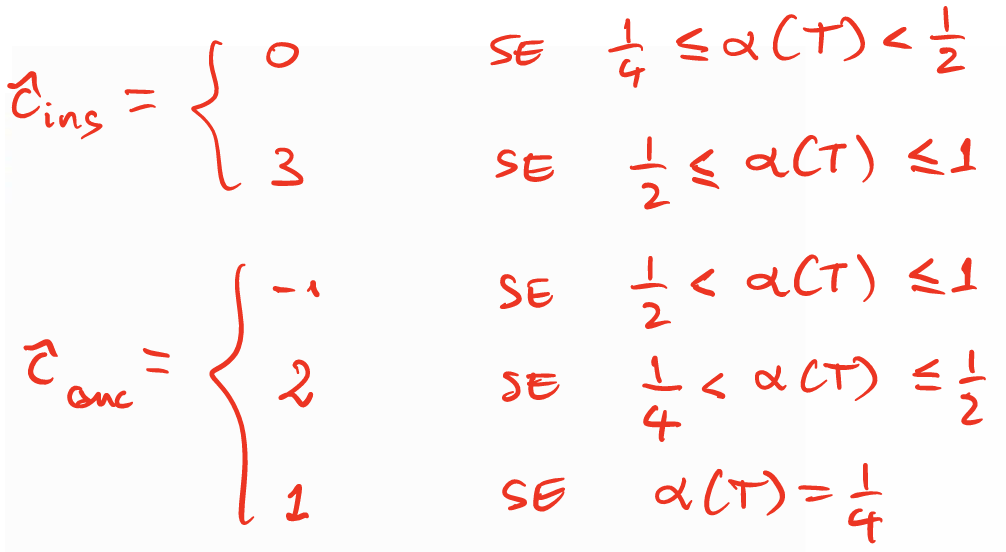
\includegraphics[width=0.8\linewidth]{Images/capitolo_1_2/costi_tabelle_dinamiche.png}
    \label{fig:costi_tabelle}
\end{figure}
In base a ciò sappiamo che $c'_{ins}\leq3,c'_{canc}\leq2<3$ da cui $T(n) \leq \sum_i^n c_i' \leq 3n$

\section{Scalare i costi}
Analizzando alcune strutture dati con il metodo del potenziale, ci potremmo trovare a situazioni in cui i conti potrebbero non tornare per qualche tipo di variabile che spesso può essere aggiustata \textbf{scalando i costi}. Vediamone un esempio.
Immaginiamo uno stack multipop con i costi:
\[c_{push} = 1 \quad c_{pop} = k \quad c_{multipop} = k s\]

Con k costante. Immaginiamo di analizzare questo con il metodo del potenziale e, visto che stiamo valutando la stessa struttura dati di prima, potrebbe venirci in mente di utilizzare come funzione $\phi(S)=|S|$, per cui avremo che:
\begin{align*}
    &c'_{push} = c_{push}+\Delta\phi=2\\
    &c'_{pop} = c_{pop} + \Delta\phi = k-1\\
    &c'_{multipop} = c_{multipop} + \Delta\phi = ks-s = (k-1)s = \Theta(s)
\end{align*}
Per cui, la complessità non risulterebbe essere quella già vista prima. Proviamo ad aggiustare i conti. Notiamo che il problema nei conti è proprio quel k in ks che non si elimina, per cui, utilizziamo come funzione potenziale $\phi(S)=k|S|$. Proviamo ora:
\begin{align*}
    &c'_{push}= c_{push} + \Delta\phi = k+1\\
    &c'_{pop} = c_{pop} + \Delta\phi = 0\\
    &c'_{multipop} = c_{multipop} + \Delta\phi=ks-ks = 0 
\end{align*}

Che dimostra di avere complessità $O(n)$.

\section{Algoritmi Online vs Algoritmi Offline}
Definiamo un algoritmo come \textbf{offline} se questo ha l'intera sequenza di input già prima che inizi l'elaborazione mentre definiamo un algoritmo \textbf{online} se gli input possono arrivare durante l'elaborazione dei dati. Se ci pensiamo, questa differenza risulta fondamentale poiché gli algoritmi offline, sapendo già tutto ciò che devono fare, possono ottimizzare al meglio il loro processo, cosa che invece gli algoritmi online non possono fare. Questo comporta che gli algoritmi online debbano necessariamente cercare di adoperare soluzioni che sono buone in quel momento nella speranza che lo siano anche per il futuro. 

Per analizzare un algoritmo online si utilizza quella che viene definita come \textbf{analisi competitiva} per cui si confronta un algoritmo online con il corrispondente algoritmo offline ottimo sulla stessa $\sigma$. Si definisce \textbf{rapporto competitivo} il valore:
\[sup_\sigma=\frac{C_{online}(\sigma)}{C_{OPT}(\sigma)}\]

E questo misura quanto l'algoritmo online sia vicino a quello ottimo. Tanto più è grande questo numero, tanto peggio sarà l'algoritmo online rispetto a quello offline. Definiamo un algoritmo come \textbf{$\alpha-$competitivo} se esiste $b \ge 0$ tale che per ogni sequenza $\sigma$ abbiamo che:
\[C_{online}(\sigma) \leq \alpha C_{opt}(\sigma)+b\]
Il problema di questa analisi è che ragiona sempre nel caso peggiore e, dunque, può spesso risultare pessimistica. 
Un esempio di problema che potremmo avere è quello dell'affitto degli sci. Supponiamo di poter decidere se affittare gli sci a 1 € al giorno o comprarli una volta per tutte a 10 €. Naturalmente se sapessimo a prescindere di stare più di 10 giorni, compreremmo direttamente gli scii, tuttavia non è possibile questa cosa nel caso online mentre lo è nel caso offline.
Allo stesso modo vale per il problema della gestione delle pagine in memoria per i computer, vediamo come gli algoritmi FIFO e LRU online e deterministici siano k-competitivi rispetto all'algoritmo Békàdy ottimale che però è offline.
\section{Self-adjusting list}
Supponiamo di voler mantenere in memoria una lista doppiamente concatenata di oggetti che possono essere richiesti uno per volta e supponiamo anche di poter riordinare la lista di volta in volta per ottimizzare gli accessi futuri e minimizzare i costi. Per fare ciò, utilizziamo un algoritmo online che sfrutta un'euristica basata sul fatto che l'elemento cercato al tempo t, sarà probabilmente ricercato nuovamente nel tempo t+x per cui, lo spostiamo all'inizio della lista. Questa euristica è detta \textbf{Move to front} e, per calcolarne il costo, consideriamo la \textbf{posizione dell'elemento ricercato} + \textbf{costo degli scambi di elementi contigui}. 
Avremo quindi una struttura $L$ con in input una sequenza $\sigma=(x_1,x_2,...,x_m)$ di richieste. Ad ogni richiesta si cerca $x_i$ scorrendo la lista da sinistra a destra.
Supponiamo di avere a disposizione un algoritmo detto \textbf{foresee}, che è un algoritmo offline che "conosce il futuro" e ottimizza tutti i processi, per fungere da benchmark per la nostra analisi.
\begin{figure}
    \centering
    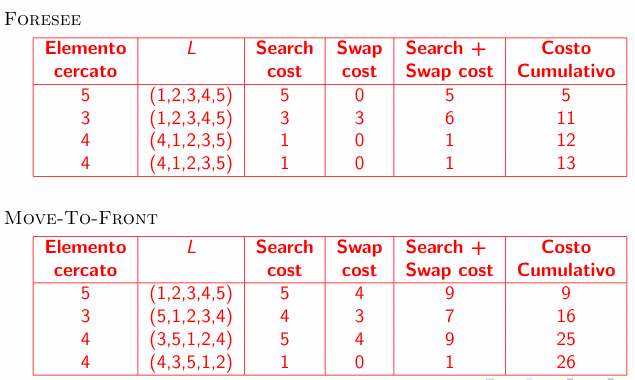
\includegraphics[width=0.5\linewidth]{Images/capitolo_1_2/prestazioni_foresee_movetofront.png}
    \label{fig:foresee_moveto}
\end{figure}

Dimostreremo che il nostro algoritmo Move-To-Front è 4-competitivo e lo faremo dimostrando che:
\[\sum_i^mc_i^M \leq 4 \sum_i^m c_i^F\]

Dove M sta per l'algoritmo Move-To-Front e F per l'algoritmo Foresee. Siano L e L' due liste contenenti gli stessi elementi, ma in ordine possibilmente diverso, definiamo una \textbf{inversione} tra L e L' una coppia non ordinata {x,y} tale che:
\[x \text{ viene prima di }y \text{ in } L \text{ ma } y \text{ precede } x \text{ in } L'\]

Indicheremo \textit{Dist}$(L,L')$ il numero di inversioni tra le due liste che rappresenta una misura di distanza tra le due. 

\begin{figure}
    \centering
    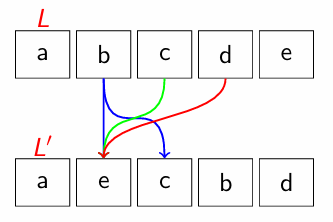
\includegraphics[width=0.5\linewidth]{Images/capitolo_1_2/inversioni_esempio.png}
    \caption{In questo esempio le coppie {b,c} {b,e} {c,e} e {d,e} sono delle inversioni}
    \label{fig:inversioni}
\end{figure}

Diamo alcune definizioni prima di effettuare un'analisi:
\begin{itemize}
    \item Sia L una lista di elementi distinti e siano m gli accessi $(x_1,...,x_m)$.
    \item Sia $L^M$ la lista di MTF e sia $L^F$ quella mantenuta da Foresee a partire dalla medesima configurazione L.
    \item Siano $L_i^M, L_i^F$ le configurazioni delle rispettive liste dopo l'i-esima operazione. 
\end{itemize}

Avremo inizialmente $L_0^M = L_0^F=L$ e mostreremo quanto detto prima cioè che $\sum_i^mc_i^M \leq 4 \sum_i^m c_i^F$. 

Facciamo un esempio completo e supponiamo di voler fare la ricerca dell'elemento x:
\begin{figure}
    \centering
    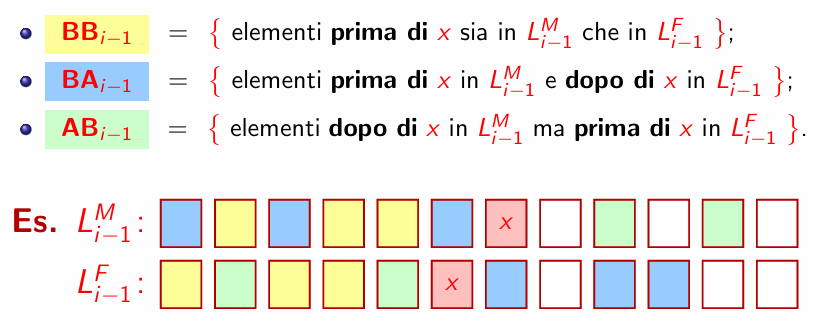
\includegraphics[width=0.5\linewidth]{Images/capitolo_1_2/mtf_competitiva.png}
    \label{fig:gruppi_mtf}
\end{figure}

In questo caso, analizzando cosa succede nel caso della lista $L_{i-1}^M$ se x passa alla prima posizione, noteremo come cambieranno le cardinalità di alcuni gruppi:
\begin{itemize}
    \item il gruppo BB cambierà poiché adesso tutti gli elementi che erano prima di x in entrambi saranno adesso dopo di x in $L_{i-1}^M$ ma prima di x rispetto a $L_{i-1}^F$;
    \item il gruppo BA cambia perché gli elementi che erano prima di x in $L_{i-1}^M$ e dopo di x in $L_{i-1}^F$, adesso saranno dopo x in entrambi;
    \item Il gruppo AB resterà invece invariato.
\end{itemize}

Sappiamo anche che: 
\begin{align*}
    &r_{L^M_{i-1}}(x) = |BB| +|BA| +1 \\
    &r_{L^F_{i-1}}(x) = |BB| +|BA| +1 \\
    &Dist(L_i^M,L_{i-1}^F)-Dist(L_{i-1}^M,L_{i-1}^F) = |BB|-|BA|
\end{align*}\footnote{$r_{L_{i-1}}(x)$ rappresenta il rango/la posizione dell'elemento x}
Inoltre: 
\begin{align*}
    &c_i^M = 2r_{L^M_{i-1}}(x)-1 \quad  \text{la posizione dell'elemento più il numero di scambi}\\
    &c_i^F \ge r_{L^F_{i-1}}(x)+s_i^F \quad \text{$s_i^F$ rappresenta il numero di scambi fatti da Foresee}\\
    &Dist(L_i^M,L_i^F)-Dist(L_{i-1}^M, L_{i-1}^F) \leq s_i^F\\
    &Dist(L_i^M,L_i^F)-Dist(L_{i-1}^M, L_{i-1}^F) = \\
    &=((Dist(L_i^M,L_i^F)-Dist(L_{i}^M, L_{i-1}^F))+((Dist(L_i^M,L_{i-1}^F)-Dist(L_{i-1}^M, L_{i-1}^F))\\
    &\leq |BB| - |BA|+s_i^F
\end{align*}

Sulla base di queste considerazioni, proviamo ad utilizzare la funzione potenziale $\phi(Dist(L_i^M,L_i^F)$.
\begin{figure}
    \centering
    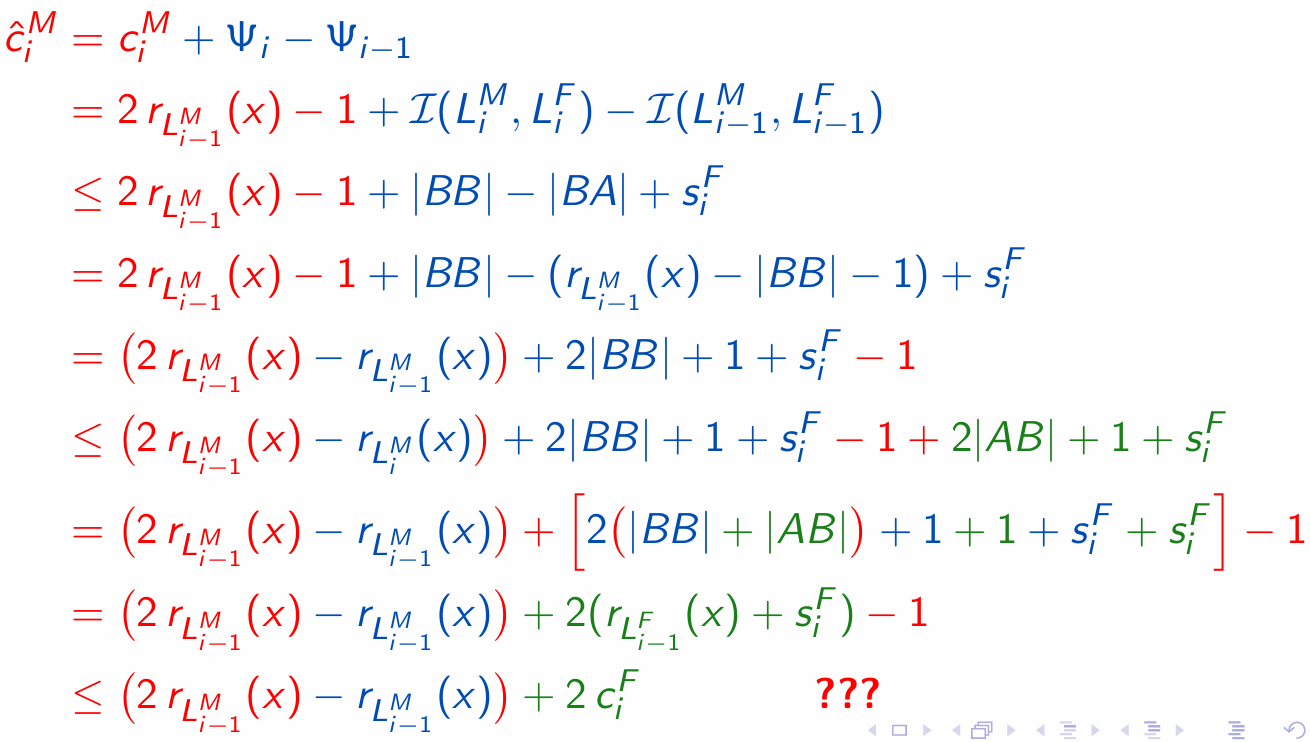
\includegraphics[width=0.5\linewidth]{Images/capitolo_1_2/mtf_primo.png}
    \label{fig:mtf_primo}
\end{figure}

In questi conti sono stati segnati in rosso ciò che deriva dal normale conto, in blu ciò che deriva dal potenziale da noi scelto e, in verde, ciò che è stato aggiunto per far quadrare i conti. Come vediamo non arriviamo al giusto risultato. Proviamo adesso a scalare il costo del potenziale e vediamo come effettivamente riusciamo nella dimostrazione.
\begin{figure}
    \centering
    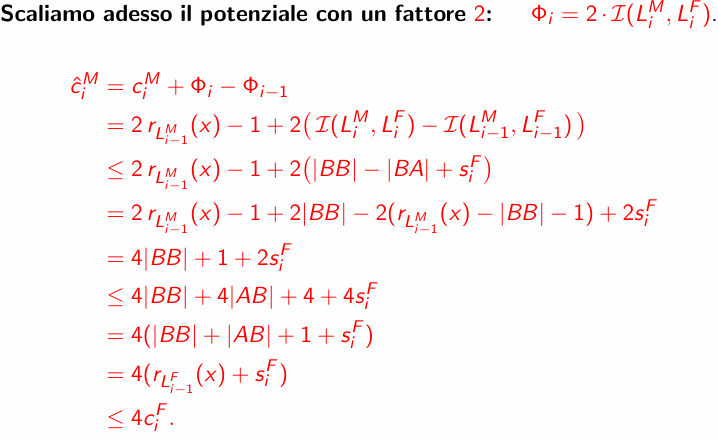
\includegraphics[width=0.5\linewidth]{Images/capitolo_1_2/mtf_secondo.png}
    \label{fig:mtf_secondo}
\end{figure}